\documentclass[11pt]{article}

\usepackage{amsmath, amssymb, amsthm}
\usepackage{tikz}

\theoremstyle{plain}
\newtheorem{thm}{Theorem}[section]
\newtheorem*{thm*}{Theorem}
\newtheorem{prop}[thm]{Proposition}
\newtheorem{lem}[thm]{Lemma}
\newtheorem*{lem*}{Lemma}
\newtheorem{dfn}[thm]{Definition}
\newtheorem{cor}[thm]{Corollary}
\newtheorem{claim}[thm]{Claim}
\newtheorem{conj}[thm]{Conjecture}
\newtheorem{ques}[thm]{Question}
\newtheorem*{rem}{Remark}


\oddsidemargin  0pt
\evensidemargin 0pt
\marginparwidth 40pt
\marginparsep 10pt
\topmargin 0pt
\headsep 10pt
\textheight 8.2in
\textwidth 6.4in
\renewcommand{\baselinestretch}{1.1}

\newcommand{\codeg}{\text{codeg}}
\newcommand{\BBE}{\mathbb{E}}
\newcommand{\BFP}{\mathbf{P}}
\usepackage{amsmath}
\usepackage{amsthm}
\usepackage{amssymb}
\usepackage{mathtools}
\usepackage{hyperref}
\usepackage{url}





\usepackage{graphicx}
\usepackage{caption}
\usepackage{subcaption}

\def\eQb#1\eQe{\begin{eqnarray*}#1\end{eqnarray*}}
\def\eQnb#1\eQne{\begin{eqnarray}#1\end{eqnarray}}
\providecommand{\e}[1]{\ensuremath{\times 10^{#1}}}
\providecommand{\pb}[0]{\pagebreak}
\DeclarePairedDelimiter\ceil{\lceil}{\rceil}
\DeclarePairedDelimiter\floor{\lfloor}{\rfloor}

\newcommand{\E}{\mathrm{E}}
\newcommand{\Var}{\mathrm{Var}}
\newcommand{\Cov}{\mathrm{Cov}}

\def\Qb#1\Qe{\begin{question}#1\end{question}}
\def\Sb#1\Se{\begin{solution}#1\end{solution}}


\newtheoremstyle{quest}{\topsep}{\topsep}{}{}{\bfseries}{}{ }{\thmname{#1}\thmnote{ #3}.}
\theoremstyle{quest}
\newtheorem*{definition}{Definition}
\newtheorem*{theorem}{Theorem}
\newtheorem*{lemma}{Lemma}
\newtheorem*{question}{Question}
\newtheorem*{preposition}{Preposition}
\newtheorem*{exercise}{Exercise}
\newtheorem*{challengeproblem}{Challenge Problem}
\newtheorem*{solution}{Solution}
\newtheorem*{remark}{Remark}
\usepackage{verbatimbox}
\usepackage{listings}
\usepackage{mathrsfs}
\date{}
\title{\vspace{-0.7cm}
Diff Geo II: Problem Set III}

\author{
Youngduck Choi 
\thanks{Department of Mathematics, Courant Institute of Mathematical Sciences, 
yc1104@nyu.edu; If you find an error and want to share with me, 
you can reach me via email.
}}

\begin{document}

\maketitle

\begin{abstract}
This work contains solutions for the problem set III.
\end{abstract}


\begin{question}[1-1]
\hfill
\begin{figure}[h!]
  \centering
    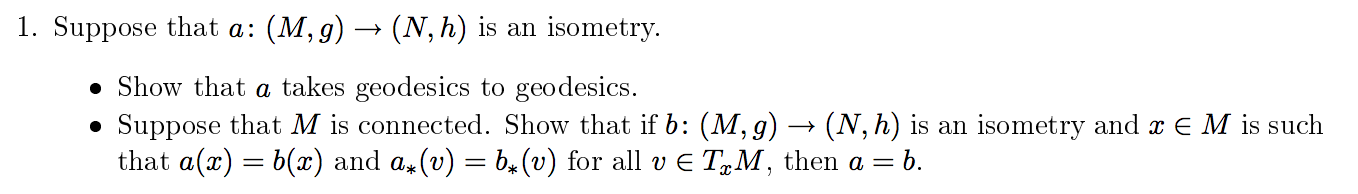
\includegraphics[width=0.7\textwidth]{dg-s3-p1.png}
\end{figure}
\end{question}
\begin{solution} \hfill \\
Let $\gamma$ be a geodesic in $M$. Then,
\eQb
D_{t(\gamma)} \dot{\gamma} &=& 0.
\eQe
As $a$ is an isometry, and $a_*$ is linear,
\eQb
D_{t(a \circ \gamma)} \dot{a \circ \gamma} = a_*( D_{t(\gamma)} \dot{\gamma}) = 0, 
\eQe
because local isometries preserve metric tensor components, and Chirstoffel symbols 
in coordinates. Hence, $a \circ \gamma$ is a geodesic. 

\bigskip

\noindent Let $U = \{q \in M : da = db\}$. Note that $U$ is closed, and $p \in U$. But,
$A$ is open, since for any $q \in U$, any normal neighborhood of $q$, $N$, must be
contained in $U$, as for any $s \in N$, there exists $v \in TqM$, such that
$\gamma_{V}(1) = r$, so
\eQb
a(r) = \gamma_{da(v)}(1) = \gamma_{db(v)}(1) = b(r).
\eQe
Hence $U$ is clopen, and $U = M$. \hfill $\qed$ 


\end{solution}

\newpage

\begin{question}[1-2]
\hfill
\begin{figure}[h!]
  \centering
    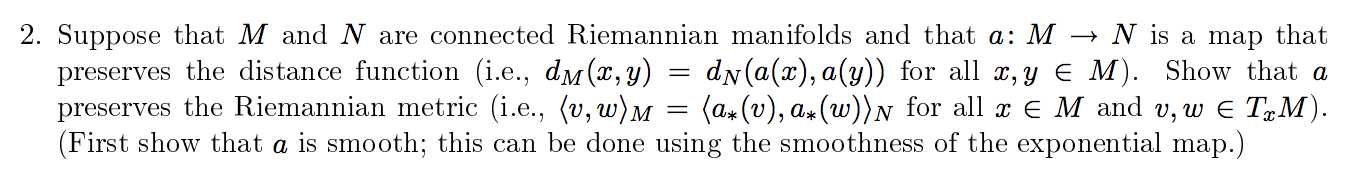
\includegraphics[width=0.7\textwidth]{dg-s3-p2.png}
\end{figure}
\end{question}
\begin{solution} \hfill \\
Suppose for the moment that $a$ is smooth. 
Let $v \in TM$, and set $\gamma(t) = exp_p(tv)$. For $t$ small enough, we know that
$\gamma$ has a constant speed. Therefore, 
\eQb
|v| |t-s| &=& d_M(\gamma(t), \gamma(s)) = d_N(F \circ \gamma(t), F \circ \gamma(s))  
\eQe
for any $t,s$ small enough. Hence,
\eQb
|Da(v)| &=& |\dfrac{d(F \circ \gamma)}{dt}|_{t = 0} 
= \lim_{t \downarrow 0} \dfrac{d_M(\gamma(t), \gamma(0))}{|t|} = |\dot{\gamma}(0)|
= |v|. 
\eQe
Therefore, $a$ is a Riemannian isometry, if we show that $a$ is smooth. 
For now, assume that $a$ is in fact bijective, which is necessary. 
Let $p \in M$. and $q = a(p)$. Then, at $q$ choose a radial coordinate from a normal
neighborhood $(r_{q_1},...,r_{q_n})$, and choose $a(p_i) = q_i$ for all $i$. Then,
\eQb
r_{q_i} \circ a(x) &=& d(a(x),q_i) = d(x,p_i)
\eQe
for all $x$. By distance preserving property, we can choose $p_i$ and $q_i$
such that $r_{p_i}(x) = d(x,p_i)$ is smooth at $p$ for all $i$. Hence,
$r \circ a$ is smooth at $p$, so $a$ is smooth. \hfill $\qed$

\bigskip

\noindent 
 
\end{solution}

\newpage

\begin{question}[1-3]
\hfill
\begin{figure}[h!]
  \centering
    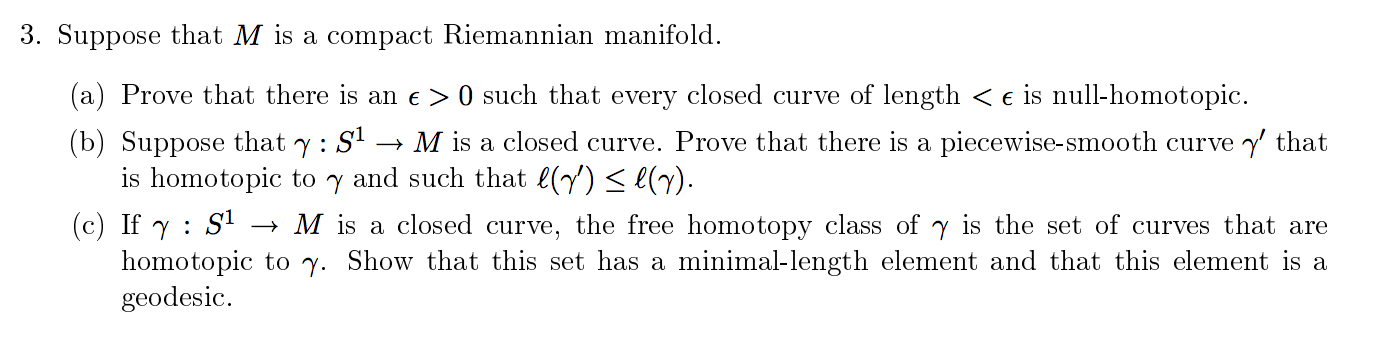
\includegraphics[width=0.7\textwidth]{dg-s3-p3.png}
\end{figure}
\end{question}
\begin{solution} \hfill \\
\textbf{(a)}
Consider the cover of $M$ obtained by for each point $p \in M$, choose 
a uniformly normal neighborhood of $p$. Then, via compactness, we can 
extract a finite subcover from the cover, which we denote by $\{N_i\}_{i \leq n}$.
Now, set $\epsilon = \dfrac{1}{2}\min_{i} \epsilon(N_i)$, 
where $\epsilon(N_i)$s are chosen
such that for each i, and each point in $N_i$ 
is contained in a geodesic ball of radius
$\epsilon(N_i)$. Then, by corollary 6.11 from John M lee, we know that
the Riemmanian distance and the radial distance are the same, so any 
closed curve of length $\epsilon$ must lie inside a geodesic ball. Therefore,
for any closed curve $\gamma$ of length less than $\epsilon$, 
we can find $\exp_p$ such that 
$\exp_p^{-1}(\gamma)$ maps into $B(0,\epsilon)$ in $T_pM$ and $\gamma(0) = p$. 
With the homotopy map 
\eQb
H(s,t) &=& s exp_p^{-1} \gamma(t) 
\eQe 
for $s,t \in [0,1]\times[0,1]$, we see that ${\exp_p}^{-1}(\gamma)$ is nulhomotopic.
Since $\exp_p$ is a diffeomorphism, so it is a homeomorphism, and we see that
$\gamma$ is nulhomotopic as well. 

\bigskip

\noindent \textbf{(b)} We cover the gamma with finitely many uniformly normal 
neighborhoods. On the lifted paths, we can do a straight line homotopy 
with the straight line from the origin to $\exp_p(\gamma(1))$. Then, the inverse
image of the homotopic path pieced together will form a piecewise smooth curve,
that is still homotopic to $\gamma$. Since the Riemmanian distance is same as
the radial function, in normal neigbhorhods, and we have chosen to do a straight 
line homotopy with the striaght line from the origin to $\exp_p(\gamma(1))$,
$L(\gamma') \leq L(\gamma)$.

\bigskip

\noindent \textbf{(c)} We denote the free homotopy class of $\gamma$ as 
$\mathfrak{H}$, and set $L = \inf_{\gamma' \in 
\mathfrak{H}} L(\gamma')$. From (b), we can choose a minimizing sequence 
$\{\gamma_n\} \subset \mathfrak{H}$ such that $\gamma_n$ is piecewise smooth,
and unit speed. Then, 
\eQnb
d(\gamma_n(t_1),\gamma_n(t_2)) &\leq& L(\gamma_n|_{[t_1,t_2]}) \label{eq:3-3-1} \\ 
&\leq& |t_1 - t_2| \label{eq:3-3-2} 
\eQne  
for each $n$ and $t_1, t_2 \in S^1$, where~\eqref{eq:3-3-1} holds by definition
of Riemmanian distance, and~\eqref{eq:3-3-2} holds by the choice of unit speed
parametrization, Therefore, $\{\gamma_n\}$ are $1-$Lipschitz family. Furthermore,
for any metric ball in $S^1$, denoted by $B$,
\eQb
\gamma_n(B) \subset M
\eQe 
for each $n$ trivially, so by Arzela-Ascoli, we can extract a subsequence, which 
we still denote as $\{\gamma_n\}$, converges uniformly to some $\gamma^*$. We now
claim that the $\gamma^*$ is homotopic to $\gamma$, $L(\gamma^*) = L$, and geodesic.
Using the uniformly normal covering as in a, and via compactness, we can have 
some small $\delta > 0$, such that for each $p \in M$, there exists a geodesic ball
of radius $\delta$. Now, choose $\gamma_{n_0}$ from $\{\gamma_n\}$ such that
$\gamma_{n_0}$ is uniformly $\dfrac{\delta}{2}$ away from $\gamma^*$. Then, we see that
we can form a piecewise homotopy between $\gamma_{n_0}$ and $\gamma^*$
with finite number of geodesic balls, using straight line homotopy available at 
the tangent spaces. This shows that the uniform convergence preserves the property of
being homotopic to $\gamma$, so $\gamma^*$ is homotopic to $\gamma$. Now, 
to prove that $\gamma^*$ is indeed a minimal length element, since 
$L(\gamma_n) \to L$, it suffices to show that $L(\gamma_n) \to L(\gamma)$, which is
equivalent to 
\eQb
\int_{S_1} |\dot{\gamma_n}(t)| dt &\to& \int_{S_1} |\dot{\gamma^*}(t)| dt.
\eQe 
Since each $\gamma_n$ is piecewise smooth, and $\gamma_n$ converges uniformly
$\gamma$, we formally expect that 
\eQb
|\dot{\gamma_n}(\cdot)| &\to& |\dot{\gamma^*}(\cdot)| \>\>\> \text{almost everywhere}. 
\eQe 
and $\dot{\gamma_n}(\cdot)$ are $L^1$. Then, by DCT, we would have the desired conclusion.
The limit object should be locally minimizing curve, which implies that it is a geodesic.
\hfill $\qed$ 
\end{solution}

\end{document}
